\documentclass[a4paper]{article}

\usepackage[francais]{babel}
\usepackage[utf8]{inputenc}
\usepackage[OT1]{fontenc}
\usepackage{amsmath}
\usepackage{amssymb}
\usepackage{graphicx}
\usepackage{url}
\usepackage{subfigure}

\graphicspath{ {./imgs/} }

% shorten margin
\usepackage[]{fullpage}

\title{Configuration et sécurisation de services réseaux}
\author{Mathieu BIVERT, Sophie VALENTIN}

\makeatletter
\def\thickhrulefill{\leavevmode \leaders \hrule height 1pt\hfill \kern \z@}
\def\maketitle{
	\null
	\thispagestyle{empty}
	\vskip 1cm
	\begin{center}
		\normalfont\large\huge\@author
	\end{center}
	\vfil
	\vfil
	\vfil
	\vfil
	\vfil
	\vfil
	\vfil
	\vfil
	\vfil
	\vfil
	\vfil
	\hrule height 2pt
	\par
	\begin{center}
				\huge \strut \@title \par
				\@date
	\end{center}
	\hrule height 2pt
	\par
	\vfil
	\vfil
	\vfil
	\vfil
	\vfil
	\vfil
	\vfil
	\vfil
	\vfil
	\vfil
	\vfil
	\vfil
	\vfil
	\vfil
	\vfil
	\vfil
	\vfil
	\vfil
	\vfil
	\vfil
	\vfil
	\vfil
	\vfil
	\vfil
	\vfil
	\begin{center}
  			\huge Professeur : Bruno MARTIN
    \end{center}
	\null
	\begin{figure}[!ht]
		\centering
		
\includegraphics[scale=.5]{polytech.png}
	\end{figure}
	\vfil
	\cleardoublepage
}
\makeatother

\begin{document}
\maketitle

\newpage
\tableofcontents

\newpage

\section{Scénario}
Serveur « public » fournissant accès distant (VPN), compte email
(postfix, dovecot, client email), espace web (apache).

Encryption autant que faire ce peut.

Logs.

Outils d'audit.

\section{Topologie}
\section{Mise en place d'une passerelle et accès à Internet}
Une passerelle (gateway) est un homme du milieu reliant
deux réseaux distincts. Dans le cas présent, la machine \textit{passerelle}
doit faire communiquer les deux réseaux SLAN (192.168.1.0/24) et LAN Travaux 
Pratiques (192.168.2.0/24).

La passerelle doit être capable de transmettre des paquets IP :
\begin{verbatim}
  (passerelle)# echo 1 > /proc/sys/net/ipv4/ip_forward
\end{verbatim}

Afin de maintenir l'\textit{IP forwarding} après un reboot de la machine
\textit{passerelle}, on décommente dans le fichier \textit{/etc/sysctl.conf}
la ligne suivante :
\begin{verbatim}
  #net.ipv4.ip_forward=1
\end{verbatim}

\vspace{1\baselineskip}
L'IP Masquerade (Network Address Translation) doit être
activée. Cette fonctionnalité modifie les entêtes IPs du trafic
passant par \textit{passerelle} afin de rendre invisibles, au niveau IP,
les machines de LAN Travaux Pratiques depuis l'extérieur.
Ici on utilise du NAT dit de source utilisant la chaîne 
\textit{POSTROUTING} puisqu'on modifie les adresses sources du paquet.
\begin{verbatim}
  (passerelle)# iptables -t nat -A POSTROUTING -o eth0 -s 192.168.2.0/24 -j MASQUERADE
\end{verbatim}

Note : L'interface \textit{eth0} est connectée au réseau SLAN.

\vspace{1\baselineskip}
Enfin, syslogd doit être activé afin de logger les activités d'iptables

\begin{verbatim}
  (passerelle)# apt-get install inetutils-syslogd
  (passerelle)# edit /etc/syslog.conf # logs dans /var/log/kernel.log
  (passerelle)# services syslog
\end{verbatim}

\subsection{Tests}
On choisit un client, par exemple \textit{client-bsd}. On lui
retire l'interface réseau connectée à SLAN \textit{em0}, et on s'assure que
la machine est bien connectée sur LAN Travaux Pratiques via \textit{em1}, et
qu'elle peut communiquer avec la passerelle. 
\begin{verbatim}
  (client-bsd)# ifconfig em0 down
  (client-bsd)# ifconfig em1
  (client-bsd)# ping passerelle.cs.sr
\end{verbatim}

\vspace{1\baselineskip}
Puis, on configure la table de routage du client afin
que la route par défaut passe par \textit{passerelle} et on vérifie :
\begin{verbatim}
  (client-bsd)# netstat -r
\end{verbatim}
\begin{figure}[!ht]
	\centering
	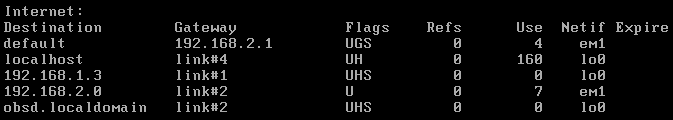
\includegraphics[scale=.5]{Internet.png}
	\caption{\label{routes} Table de routage de \textit{client-bsd}}
\end{figure}

\vspace{1\baselineskip}
Enfin, on s'assure qu'il est possible de contacter le serveur
 et d'atteindre Internet.
\begin{verbatim}
  (client-bsd)# ping -c3 google.fr
\end{verbatim}

\vspace{1\baselineskip}
On vérifie les logs sur la passerelle:
\begin{verbatim}
  (passerelle)# tail -f /var/log/kernel.log
\end{verbatim}

nmap ? Faire peut-être une partie "outils d'attaque et... d'audit"
où on explique l'utilisation de nmap, metasploit, vas (TP de demain)
et en quoi ils nous aident à sécu notre propre réseau.

\section{Mise à disposition d'un accès distant sur la machine et sécurisation}
Telnet, SSH, VPN
Expliquer comment mettre en place TCP Wrapper avec Telnet mais pas sécurisé.
essai ssh avec mitm? (normalement il affiche un message du genre
"SOMEONE MAY BE ON THE CABLE!")

\subsection{Serveur Telnet et attaques de \textit{sniffing}}

On commence par installer un serveur \textit{telnet} afin d'offrir
un premier accès distant à la machine \textit{passerelle}.

On n'utilisera pas ici le démon classique de telnet mais un démon
générique nommé \textit{inetd} permettant de minimiser le nombre
de processus lancés. Quand \textit{inetd} reçoit une demande 
de connexion, il lance le processus serveur adéquat. 

Pour ce faire, on installe le serveur telnet.
\begin{verbatim}
  (passerelle)# apt-get install telnetd
\end{verbatim}

Puis, on modifie le fichier \textit{/etc/inetd.conf} pour y
ajouter le service \textit{telnet} dans la section des services
standard, de façon à ce qu'il soit démarré automatiquement
en tant qu'utilisateur telnetd:
\begin{verbatim}
  (passerelle)# grep '^telnet' /etc/inetd.conf
  telnet        stream    tcp nowait telnetd /usr/sbin/tcpd /usr/sbin/in.telnetd
\end{verbatim}

\vspace{1\baselineskip}
On va maintenant tenter d'intercepter le couple \textit{login/passwd}
lors d'une connexion \textit{telnet} entre \textit{client-bsd}
et \textit{passerelle}.

Pour opérer, on utilise l'outil \textit{ettercap} depuis la machine BackTrack. 
Il faut le lancer ainsi :
\begin{verbatim}
  (backtrack)# ettercap -G
\end{verbatim}

\begin{enumerate}

\item Dans le menu, on clique tout d'abord sur \textit{Sniff} et on sélectionne 
\textit{Unified sniffing} avant de choisir l'interface \textit{eth1}
qui est sur LAN Travaux Pratiques.

\item Dans le menu \textit{Hosts}, on lance un scan du réseau local puis
depuis le même menu, on affiche la liste des hôtes.

\begin{figure}[!ht]
	\centering
	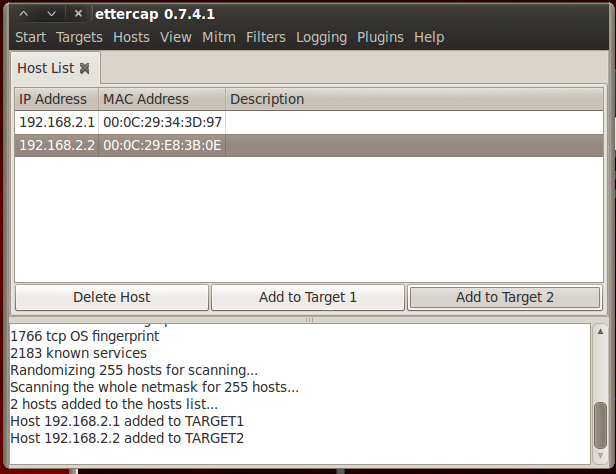
\includegraphics[scale=.4]{Hosts.PNG}
	\caption{\label{hosts} Hôtes détectés par le scan}
\end{figure}

On reconnaît les adresses IP de \textit{passerelle} et 
\textit{client-bsd}. Il suffit donc de spécifier que ce sont
nos deux cibles avec les boutons \textit{TARGET 1} et \textit{TARGET 2}.

\item Comme il s'agit d'un réseau commuté, on doit empoisonner les tables
ARP (\textit{ARP poisoning}) avant de lancer le \textit{sniffing} pour
récupérer le trafic entre les deux cibles.

Dans le menu \textit{Mitm}, on sélectionne donc \textit{ARP Poisoning}.

\item Enfin, on sélectionne dans le menu \textit{Start} le choix \textit{Start Sniffing}.

\end{enumerate}

La machine \textit{client-bsd} se connecte avec \textit{telnet}.

\begin{figure}[!ht]
	\centering
	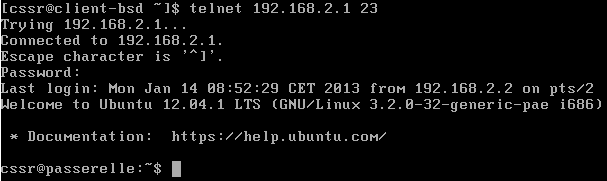
\includegraphics[scale=.5]{Telnet.PNG}
	\caption{\label{hosts} Connexion à \textit{passerelle}}
\end{figure}

Et on constate qu'il est extrêmement facile d'obtenir le couple \textit{login/password} en clair:

\begin{figure}[!ht]
	\centering
	
\includegraphics[scale=.5]{Telnet_passwd.png}
	\caption{\label{hosts} Couple en clair}
\end{figure}

On ne veut donc pas proposer un service d'accès à distance non sécurisé, c'est-à-dire
basé sur des communications transmises en clair sur le réseau. 

 
\subsection{Serveur SSH  et optimisations}
SSH (Secure SHell) joue un rôle similaire à telnet, mais contrairement à ce
dernier, il intègre des mécanismes de sécurité, comme le chiffrement des
communications.

On installe puis démarre un serveur SSH sur la plateforme:
\begin{verbatim}
  (passerelle)# apt-get install openssh-server
  (passerelle)# service ssh start
\end{verbatim}

On teste une connexion avec mot de passe (l'option \textit{-v} est
utilisé pour montrer la différence avec une connexion à base de
clefs, voir plus bas)
\begin{verbatim}
  (client-bsd)$ ssh -v cssr@passerelle.cs.sr
  <METTRE L'OUTPUT ICI>
\end{verbatim}

Afin d'éviter d'avoir à entrer le mot de passe à chaque connexion, on peut
utiliser un système à base de clefs. On génère un couple clef privée/publique
de type RSA sur le client:
\begin{verbatim}
(client-bsd)$ ssh-keygen -t rsa
Generating public/private rsa key pair.
Enter file in which to save the key (/home/cssr/.ssh/id_rsa): 
Enter passphrase (empty for no passphrase): 
Enter same passphrase again: 
Your identification has been saved in /home/cssr/.ssh/id_rsa
Your public key has been saved in /home/cssr/.ssh/id_rsa
The key fingerprint is:
f4:3e:54:9f:df:eb:72:cc:7a:da:29:a5:79:58:0c:44 cssr@client-bsd
The key's randomart image is:
+--[ RSA 2048]----+
|            .E   |
|             .   |
|        .   o    |
|       . . . o . |
|        S o   =  |
|         o     =.|
|          o   O o|
|           . *.*o|
|             oX= |
+-----------------+
\end{verbatim}

Deux fichiers sont alors générés :
\begin{description}
	\item[id\_rsa.pub]	Clé publique devant être connue du serveur;
	\item[id\_rsa] 		Clé privée ne devant pas être dévoilée.
\end{description}

Côté serveur, on doit maintenant ajouter la clef publique sur le
serveur. SSH cherche dans le répertoire \textit{\$HOME/.ssh/} les
fichiers dont le nom commence par \textit{authorized\_keys}. Ceux-ci
doivent contenir une clef par ligne.

On transmet ainsi la clé publique sur le serveur, par exemple avec
\textit{scp}:
\begin{verbatim}
  (client-bsd)$ scp .ssh/id_rsa.pub cssr@passerelle.cs.sr:~/.ssh/authorized_keys2
\end{verbatim}

On prend soin d'ajuster les permissions du fichier :
\begin{verbatim}
  (passerelle)# chmod 700 authorized_keys2
\end{verbatim}
 
Enfin, on s'assure que l'authentification par clefs marche bien, et
qu'il est difficile de récupérer les informations sur la connexion
avec une attaque MITM.

La configuration du serveur SSH se fait dans le fichier \textit{/etc/ssh/sshd\_config}.
Il peut-être intéressant d'y faire les réglages suivants:
\begin{description}
	\item[X11Forwarding no] pour réduire le trafic X$11$, et donc réduire les
	risques de sécurité;
	\item[PermitRootLogin no] pour désactiver un accès distant direct au compte
	root;
	\item[Port 42], où tout autre port différent du port $22$ pour éviter les
	tentatives de connexions lancées par des bots (déni de service).
\end{description}

\subsection{Accès distant par VPN}

Alors que SSH permet l'accès sécurisé à une machine distante (le serveur SSH),
un VPN (Virtual Private Network) permet d'accéder au serveur VPN et à son réseau local de façon sécurisée.

On désire établir un réseau virtuel d'adresse 10.0.0.0 entre le client \textit{client-bsd} 
et le serveur \textit{passerelle}. 
On installe le paquet \textit{openvpn} sur chaque machine :
\begin{verbatim}
  (passerelle)# apt-get install openvpn
  (client-bsd)# pkg_add -r openvpn
\end{verbatim}

On effectue un premier test non chiffré.
\begin{verbatim}
  (passerelle)# openvpn --dev tun0 --ifconfig 10.0.0.1 10.0.0.2
  (client-bsd)# openvpn --remote passerelle.cs.sr --dev tun0 --ifconfig 10.0.0.2 10.0.0.1
\end{verbatim}

De chaque côté, une interface réseau \textit{tun0} apparaît : il s'agit
d'une interface "Point-à-point".
Et on fait quelques tests de connectivité dans le réseau virtuel.

\begin{figure}[!ht]
	\centering
	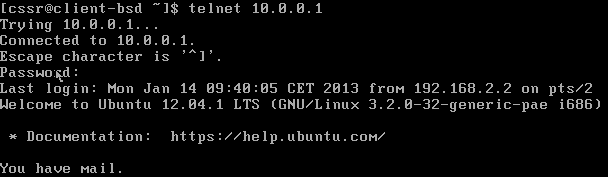
\includegraphics[scale=.6]{Telnet_VPN.PNG}
	\caption{\label{telnet_vpn} Le serveur est accessible via son interface \textit{tun0}}
\end{figure}

Un VPN a la propriété d'être privé : cela signifie que seules les entités de part et
d'autre du VPN peuvent accéder aux données en clair. Il est donc
indispensable de chiffrer les communications avec un VPN. Il existe
cependant plusieurs techniques cryptographiques.

\subsubsection{Clé partagée} 

On engendre une clé partagée sur le serveur.
\begin{verbatim}
  (passerelle)# openvpn --genkey --secret static.key
\end{verbatim}

Puis, on recopie cette clé sur \textit{client-bsd} avec la commande \textit{scp}
qui est sécurisée.

On peut relancer maintenant le client et le serveur avec les commandes suivantes.
\begin{verbatim}
  (passerelle)# openvpn --dev tun0 --ifconfig 10.0.0.1 10.0.0.2 --secret /etc/openvpn/static.key
  (client-bsd)# openvpn --remote passerelle.cs.sr --dev tun0 --ifconfig 10.0.0.2 10.0.0.1 
                --secret /etc/openvpn/static.key
\end{verbatim}

La connexion est maintenant chiffrée.

On remarque que le nombre de paramètres de la commande \textit{openvpn} devient
de plus en plus important. C'est d'autant plus le cas si on veut effectuer 
de la compression. 
Il est préférable de lancer la commande en faisant référence à un fichier de configuration.
\begin{verbatim}
  (passerelle)# openvpn /etc/openvpn/server.conf
  (client-bsd)# openvpn /etc/openvpn/client.conf
\end{verbatim}

\subsubsection{Utilisation de clés SSL/TLS}

Avec cette technique, les pairs s'authentifient entre-eux à l'aide de certificats.
Chaque pair (serveur ou un des clients) possède un certificat et une clé privée, gardée secrète.
Les différents certificats sont signés par une autorité de certification. Et dans notre cas,
l'autorité de certification est en fait le serveur.

Les scripts fournis dans la documentation d'OpenVPN permettent de construire l'AC ainsi
que les différentes paires de clés.
On commence par localiser et se déplacer dans le dossier \textit{easy-rsa/2.0}
\begin{verbatim}
  (passerelle)# cd /usr/share/doc/openvpn/examples/easy-rsa/2.0/
\end{verbatim}

On peut modifier le script \textit{vars} afin de renseigner des informations X509 du
certificat (\textit{KEY\_COUNTRY}, \textit{KEY\_PROVINCE}, \textit{KEY\_CITY}, 
\textit{KEY\_ORG} et \textit{KEY\_EMAIL}).

Et on lance les scripts suivants :
\begin{verbatim}
  (passerelle)# . ./vars
  (passerelle)# ./clean-all
  (passerelle)# ./build-ca # Génère le certificat et la clé privée de l'AC
  (passerelle)# ./build-dh # Génère les paramètres de l'échange des clés de DH
\end{verbatim}

L'avant-dernière commande a généré dans \textit{keys} les fichiers \textit{ca.crt}
et \textit{ca.key}. Quant à la dernière, elle a généré le fichier \textit{dh1024.pem}.

La commande \textit{./build-key-server passerelle} crée le certificat et la clé privée du serveur.
La commande \textit{./build-key bsd} crée le certificat et la clé privée de \textit{client-bsd} et
cette procédure doit être répétée pour chaque client du VPN.
Les deux certificats sont signés par la clé privée de l'AC que l'on a créée.

Au final on dispose des deux couples de clés dans le dossier \textit{keys} :
\begin{itemize}
  \item le certificat du serveur \textit{passerelle.crt}
  \item la clé privée du serveur \textit{passerelle.key}
  \item le certificat de \textit{client-bsd} \textit{bsd.crt}
  \item la clé privée de \textit{client-bsd} \textit{bsd.key}
\end{itemize}

On doit maintenant transmettre le certificat et la clé privée de \textit{client-bsd}
du serveur au client. On doit également transmettre le certificat de l'AC. 
Comme la clé privée est une donnée secrète, on utilise
un transfert sécurisé (par exemple avec \textit{scp}).

Dans la documentation, des fichiers de configuration exemples sont donnés.
On adapte alors \textit{server.conf} que l'on place sur \textit{passerelle}
et \textit{client.conf} placé sur \textit{client-bsd}

Dans \textit{server.conf}, on spécifie :
\begin{verbatim}
  ca /easy-rsa/2.0/keys/ca.crt # Certificat de l'AC
  cert /easy-rsa/2.0/keys/passerelle.crt
  key /easy-rsa/2.0/keys/passerelle.key  # This file should be kept secret
  dh /easy-rsa/2.0/keys/dh1024.pem
  server 10.8.0.0 255.255.255.0 
\end{verbatim}

Et dans \textit{client.conf}, on indique :
\begin{verbatim}
  remote passerelle.cs.sr 1194
  ca /easy-rsa/2.0/keys/ca.crt
  cert /easy-rsa/2.0/keys/bsd.crt
  key /easy-rsa/2.0/keys/bsd.key
\end{verbatim}

On démarre le serveur et le client :
\begin{verbatim}
  (passerelle)# openvpn /easy-rsa/2.0/server.conf
  (client-bsd)# openvpn /easy-rsa/2.0/client.conf
\end{verbatim}

\subsubsection{Démarrage automatique d'un service}

Au démarrage de la machine Linux, le processus \textit{init} 
est chargé de démarrer certains services selon le niveau de démarrage.
\textit{init} utilise des scripts \textit{shell} qui activent ou désactivent
les services. Ainsi, à chaque niveau de démarrage, \textit{init} exécute
les scripts du niveau de démarrage courant.

Les niveaux 2 à 5 correspondent au mode multi-utilisateurs. C'est le mode
par défaut sur les distributions Linux. Cependant, une distribution 
\textit{Debian} utilise le niveau 2 par défaut alors qu'une distribution
\textit{OpenSuse} utilise le niveau 5 par défaut.

Tous les scripts de démarrage sont rangés dans \textit{/etc/init.d} et
des liens y font référence depuis les répertoires de niveau de démarrage.

Ainsi, on s'assure que des liens vers le script d'OpenVPN \textit{/etc/init.d/openvpn} 
sont bien présents dans les répertoires \textit{rc2.d}, \textit{rc3.d}, \textit{rc4.d} et
\textit{rc5.d} du répertoire \textit{/etc}.
Les commentaires du script \textit{/etc/init.d/openvpn} peuvent nous conforter dans
cette idée.
\begin{verbatim}
# Default-Start:     2 3 4 5
\end{verbatim}

Le script \textit{/etc/init.d/openvpn} peut être configuré 
avec le fichier \textit{/etc/default/openvpn} et avec des fichiers
de configuration placés dans \textit{/etc/openvpn} ayant l'extension \textit{conf}.
On n'a donc pas besoin de préciser dans \textit{/etc/default/openvpn} les
arguments de la commande \textit{openvpn} puisque le script lira 
le fichier de configuration \textit{/etc/openvpn/server.conf}

Le serveur sera donc automatiquement démarré avec les bons paramètres.

\subsubsection{Pont Ethernet}

Un pont réseau travaille au niveau 2 de la couche OSI et permet de combiner
une interface Ethernet avec une (ou plusieurs) interface(s) virtuelle(s) TAP (également de niveau 2).
Ainsi on peut relier les machines du réseau virtuel créé par OpenVPN avec celles 
connectées au réseau local (ici 192.168.2.0/24). 

On souhaite mettre en place le pont côté serveur (machine \textit{passerelle})
afin que les clients du VPN soient capables de se connecter au pont. Ils recevront
une adresse du réseau local grâce au serveur OpenVPN qui leur affectera une adresse
IP de son \textit{pool} d'adresses.

On commence par installer \textit{bridge-utils}.
\begin{verbatim}
  (passerelle)# sudo apt-get install bridge-utils
\end{verbatim}

On prend soin de déplacer les scripts \textit{bridge-utils} et \textit{bridge-stop}
dans \textit{/etc/openvpn}. Et on modifie \textit{bridge-start} ainsi :
\begin{verbatim}
  br="br0"
  tap="tap0"
  eth="eth1"
  eth_ip="192.168.2.1"
  eth_netmask="255.255.255.0"
  eth_broadcast="192.168.2.255"
\end{verbatim}

On lance ensuite le script : les interfaces \textit{tap0} et \textit{br0} sont ajoutées.
Puis, il faut modifier le script \textit{/etc/openvpn/server.conf} pour qu'il tienne 
compte du pont Ethernet.
Ainsi on remplace
\begin{verbatim}
  dev tun
\end{verbatim}
par
\begin{verbatim}
  dev tap0
\end{verbatim}

Et on remplace
\begin{verbatim}
  server 10.8.0.0 255.255.255.0
\end{verbatim}
par
\begin{verbatim}
  server-bridge 192.168.2.1 255.255.255.0 192.168.2.128 192.168.2.254
\end{verbatim}

Le \textit{pool} des adresses IP distribuées est alors la plage 192.168.2.128 - 192.168.2.254.

Depuis les derniers noyaux, les trames Ethernet contenant des paquets IP qui passent
par un pont sont soumises aux règles \textit{iptables}.
Afin d'autoriser le trafic du tunnel, on applique donc :
\begin{verbatim}
  (passerelle)# iptables -A INPUT -i tap0 -j ACCEPT
  (passerelle)# iptables -A INPUT -i br0 -j ACCEPT
  (passerelle)# iptables -A FORWARD -i br0 -j ACCEPT
\end{verbatim}
Note : l'\textit{ip\_forwarding} est déjà activé.

Avant de démarrer le service \textit{openvpn}, il faut démarrer \textit{bridge-start}.
Et après avoir stoppé \textit{openvpn}, il faut lancer \textit{bridge-stop}.

Côté client, on remplace
\begin{verbatim}
  dev tun
\end{verbatim}
par
\begin{verbatim}
  dev tap
\end{verbatim}

Par défaut, un noyau \textit{bsd} ne prend pas en charge les interfaces Ethernel virtuelles (\textit{tap}).
Il faut donc charger le module :
\begin{verbatim}
  (client-bsd)# kldload if_tap
\end{verbatim}

Pour rendre cela persistant, on ajoute dans \textit{/boot/loader.conf} :
\begin{verbatim}
  if_tap_load="YES"
\end{verbatim}

On démarre le client \textit{openvpn} et on vérifie qu'on réussit rien à atteindre
l'interface \textit{eth1} de \textit{passerelle}. Le pont est correctement établi.
On ne triche pas puisque dans des manipulations précédentes, l'interface \textit{em1}
de \textit{client-bsd} qui était connectée au réseau 192.168.2.0/24 a été désactivée.

\section{Configuration d'un serveur web et d'OpenSSL}
\subsection{Installation d'OpenSSL}
\begin{verbatim}
  (passerelle)# ./configure --prefix=/usr/local && make && make install
  (passerelle)# cat >> /etc/ld.so.conf
  /usr/local/openssl/lib
  ^D
  (passerelle)# ldconfig
\end{verbatim}

\subsection{Installation d'Apache2}
Après avoir récupéré les sources sur le site (et vérifié le hash du fichier), on configure
Apache avec le support d'OpenSSL
\begin{verbatim}
  (passerelle)# ./configure --option-du-chemin-ssl=/usr/local/openssl --prefix=/usr/local/apache2
  (passerelle)# /usr/local/bin/apache2/bin/apachectl start
  (passerelle)# nc passerelle 80
  GET /
  <html><body><h1>It works!</h1></body></html>
\end{verbatim}

\subsection{Génération d'un certificat $X509$}
On génère dans l'ordre:
\begin{enumerate}
	\item une cléf privée;
	\item un CSR (Certificate Signing Request);
	\item un certificat $X509$.
\end{enumerate}

Enfin, on copie (arbitrairement) ces fichiers dans
\textit{/usr/local/apache2/conf/}:
\begin{verbatim}
(passerelle)# openssl version
OpenSSL 0.9.8x 10 May 2012
(passerelle)# openssl req -new -key ca.key -out ca.csr
You are about to be asked to enter information that will be incorporated
into your certificate request.
What you are about to enter is what is called a Distinguished Name or a DN.
There are quite a few fields but you can leave some blank
For some fields there will be a default value,
If you enter '.', the field will be left blank.
-----
Country Name (2 letter code) [AU]:FR
State or Province Name (full name) [Some-State]:France
Locality Name (eg, city) []:Nice
Organization Name (eg, company) [Internet Widgits Pty Ltd]:CSSR Ltd
Organizational Unit Name (eg, section) []:
Common Name (e.g. server FQDN or YOUR name) []:
Email Address []:

Please enter the following 'extra' attributes
to be sent with your certificate request
A challenge password []:A challenge password
An optional company name []:
(passerelle)# openssl x509 -req -days 365 -in ca.csr -signkey ca.key -out ca.crt
Signature ok
subject=/C=FR/ST=France/L=Nice/O=CSSR Ltd
Getting Private key
(passerelle)# cp ca.* /etc/ssl/
\end{verbatim}

Le certificat pourra être utilisé par les serveurs HTTPS, SMTP, IMAPS, etc.

\subsection{Passage à HTTPS}
On inclu le fichier \textit{extra/httpd-ssl.conf} depuis le
\textit{httpd.conf}:
\begin{verbatim}
Include conf/extra/httpd-ssl.conf
\end{verbatim}

Puis, on règle les chemins vers le certificat et la clef dans ce
dernier:
\begin{verbatim}
SSLCertificateFile "/usr/local/apache2/conf/ca.crt"
SSLCertificateKeyFile "/usr/local/apache2/conf/ca.key"
\end{verbatim}

Enfin, on règle les paramètres pour le domaine virtuel dans lequel
tourne la partie HTTPS:
\begin{verbatim}
DocumentRoot "/export/wwws/"
ServerName www.example.com:443
ServerAdmin you@example.com
ErrorLog "/usr/local/apache2/logs/error_log"
TransferLog "/usr/local/apache2/logs/access_log"

<Directory /export/wwws/>
    Options FollowSymLinks
    AllowOverride None
    Order deny,allow
    #Deny from all
</Directory>
\end{verbatim}

\subsection{Tests}
Le script d'authentification fourni peut être étendu pour
fournir une interface de création de compte sur la passerelle.
On peut ainsi créer automatiquement un compte UNIX, un espace
web personnel, etc. Pour plus de sécurité, on peut se contenter
d'envoyer un email à l'administrateur de la machine avant la
création du compte, pour que celui-ci s'assure que l'utilisateur
a bien de bonnes raisons de demander un accès.

Dans tout les cas, une attaque sur le serveur sécurisé avec
ettercap fonctionne comme les attaques précèdentes (ARP spoofing)
au détail près qu'ettercap génère un faux certificat de façon
à récupérer les données d'authentification.

Un utilisateur averti risque de le remarquer, à moins que cela
soit sa première connexion sur le site. En effet, le certificat
étant auto-signé, il devra au moins être ajouté manuellement
la première fois.
\section{Service de messagerie électronique et sécurisation}
\begin{figure}[!ht]
	\centering
	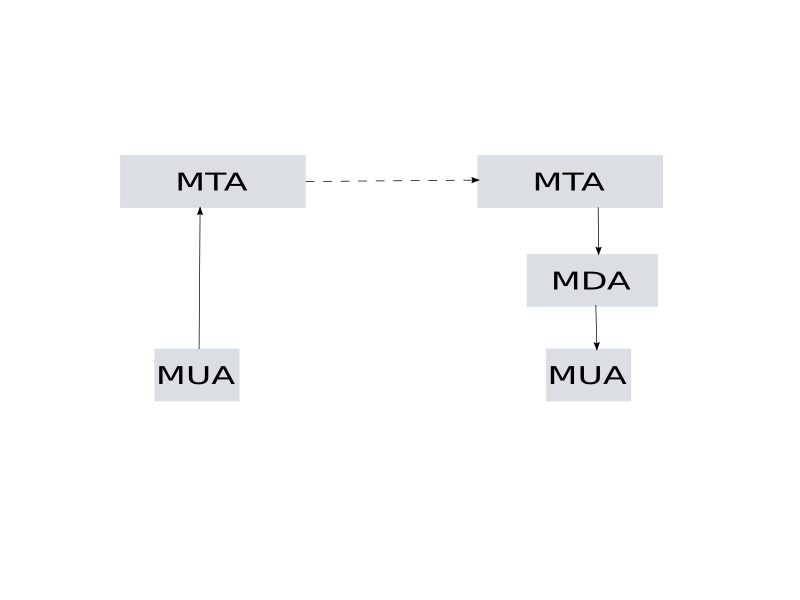
\includegraphics[scale=.5]{emailrouting.png}
	\caption{\label{emailrouting} Un MUA envoie un email à un MTA, qui
		le forward jusqu'à un MTA final, qui le transmet à un MDA.
		Enfin, le MUA du destinataire récupère l'email depuis ce MDA}
\end{figure}

La figure \ref{emailrouting} donne un exemple simple de routage d'email,
faisant intervenir $3$ pièces logicielles:
\begin{description}
	\item[MTA] Mail Transfer Agent (eg. serveur SMTP), qui relaye les
		emails de domaines en domaines jusqu'à arriver à bonne destination;
	\item[MDA] Mail Delivery Agent (eg. serveur IMAP(s)), qui reçoit les emails
		du MTA du domaine et les délivre aux MUAs qui lui demandent;
	\item[MUA] Mail User Agent c'est le client email, dont le rôle principal
		est de récupérer les emails depuis un MDA, et d'en envoyer à un MTA;
\end{description}
D'autres agents optionnels peuvent venir s'y greffer.

En pratique, on installe et configure postfix sur \textit{passerelle}.

\subsection{Envoi et transfert d'emails avec Postfix (MTA)}

Postfix est un serveur SMTP modulaire et complexe.

On installe le paquet \textit{postfix}
\begin{verbatim}
  (passerelle)# apt-get install postfix
\end{verbatim}

Une fois le paquet installé, il faut choisir la configuration de base : on choisit
"SiteInternet" afin que Postfix crée lui-même les fichiers de configuration
dans \textit{/etc} et qu'il les remplisse de quelques directives de base.

On modifie le fichier \textit{/etc/postfix/main.cf}
\begin{verbatim}
  smtpd_banner = # On ne met rien pour ne pas donner inutilement des informations
  myhostname = passerelle.cs.sr # De préférence /etc/hostname
  mydomain = cs.sr
  alias_maps = hash:/etc/aliases
  alias_database = hash:/etc/aliases

  mynetworks = 127.0.0.0/8 # Réseaux des clients de confiance
  mydestination = $myhostname, localhost.$mydomain, localhost, $mydomain # Domaines locaux
  inet_interfaces = all
\end{verbatim}

On prend soin d'exécuter le démon en mode \textit{debug} en modifiant 
dans \textit{/etc/postfix/master.cf} la ligne du service \textit{smtp} ainsi :
\begin{verbatim}
smtp      inet  n       -       n       -       -       smtpd -v
\end{verbatim}

Il faut ensuite relancer le démon.
\begin{verbatim}
  (passerelle)# /etc/init.d/postfix reload
\end{verbatim}

L'utilisateur \textit{alice} est ensuite ajouté. 
\begin{verbatim}
  (passerelle)# adduser alice
\end{verbatim}
Le mot de passe UNIX doit être précisé.

Un mail depuis l'utilisateur \textit{cssr} est envoyé à Alice.
\begin{verbatim}
  (passerelle)# echo "Hello" | mail -s Test alice
\end{verbatim}

On peut vérifier que Postfix est utilisé en visualisant les logs
dans \textit{/var/log/mail.log}

La livraison étant locale, l'agent "local" de \textit{postfix}
est utilisé. Ce dernier délègue la livraison des messages
à \textit{procmail}. On pourra donc lire le message dans 
\textit{/var/mail/alice}.
\begin{verbatim}
  (passerelle)# less /var/mail/alice
\end{verbatim}

Essayons d'envoyer un mail à un utilisateur qui n'existe pas : \textit{bob}.
La commande \textit{VRFY} du protocole SMTP nous indique qu'il n'existe pas.
\begin{figure}[!ht]
	\centering
	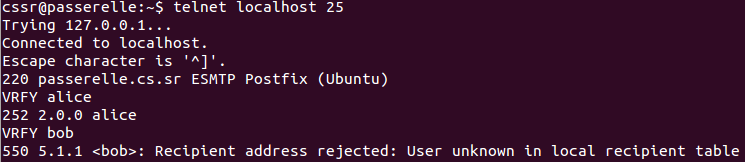
\includegraphics[scale=.6]{VRFY.PNG}
	\caption{\label{verify} Résultat \textit{VRFY}}
\end{figure}
 
On tente tout de même d'envoyer un mail avec \textit{mail}. Et 
le \textit{MAILER-DAEMON} nous répond pour nous informer que
l'email n'a pas pu être envoyé.

Avec les aliases, il est possible d'indiquer à Postfix que certains
utilisateurs locaux peuvent être redirigés vers des utilisateurs
locaux voire distants.
On souhaite ici que le courrier pour Alice.Personne soit délivré
à Alice. 
Pour ce faire, on modifie les aliases dans \textit{/etc/aliases}.
\begin{figure}[!ht]
	\centering
	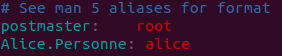
\includegraphics[scale=.7]{Aliases.PNG}
	\caption{\label{alias} Fichier des aliases}
\end{figure}

Il faut ensuite mettre à jour les aliases.
\begin{verbatim}
  (passerelle)# postalias /etc/aliases
\end{verbatim}

Et \textit{alice} reçoit bien les messages destinés à
\textit{Alice.Personne}.

On peut noter qu'il est préférable de ne pas mettre le réseau local 192.168.1.0/24 dans
\textit{mynetworks}. Effectivement, cela considère qu'il est de confiance
et qu'on peut se passer de faire des vérifications sur le nom de domaine
des destinataires. 

\subsection{Récupération d'emails avec Dovecot (MDA) et Thunderbird (MUA)}

Nous aimerions que nos utilisateurs UNIX disposent d'un système 
leur permettant de consulter et gérer à distance leurs messages.
Le protocole IMAP offre ses fonctionnalités. 

\subsubsection{Passage au format \textit{maildir}}

On utilise \textit{maildrop} au lieu de \textit{procmail}.
L'agent \textit{maildrop} sait notamment délivrer le courrier aux dossiers au format
\textit{Maildir}. L'agent \textit{procmail} délivrait, lui, le courrier
en utilisant le format \textit{mailbox} c'est-à-dire en concaténant
tous les messages dans un même fichier. \textit{Maildir} permet
d'avoir un fichier par message.
Installons donc \textit{maildrop}
\begin{verbatim}
  (passerelle)# sudo apt-get install maildrop
\end{verbatim}

Il faut modifier la configuration de Postfix (\textit{/etc/postfix/main.cf}).
\begin{verbatim}
  mailbox_command = /usr/bin/maildrop
\end{verbatim}

On crée une boîte aux lettres par utilisateur UNIX, dans leur \$HOME.
\begin{verbatim}
  (passerelle)# cd ~
  (passerelle)# maildirmake
\end{verbatim}

Et bien sûr, on recharge la configuration de Postfix.

\subsubsection{Ajout du serveur IMAP}

On installe les paquets pour Dovecot.
\begin{verbatim}
  (passerelle)# sudo apt-get install dovecot-common
  (passerelle)# sudo apt-get install dovecot-imapd
\end{verbatim}

A l'installation, un certificat et une clé privée pour Dovecot
sont générés automatiquement. Le certificat et la clé
se trouvent respectivement dans \textit{/etc/ssl/certs/dovecot.pem}
et \textit{/etc/ssl/private/dovecot.key}. Nous les utiliserons
pour activer SSL/TLS sur le serveur IMAP.

On modifie dans \textit{/etc/dovecot/dovecot.conf} la ligne 26.
\begin{verbatim}
  listen = *
\end{verbatim}

La méthode d'authentification va être modifié dans 
\textit{/etc/dovecot/conf.d/10-auth.conf}. 
On autorise le \textit{plain text} parce que
SSL/TLS sera utilisé.
\begin{verbatim}
  disable_plaintext_auth = no # ligne 9
  auth_mechanisms = plain login # ligne 97
\end{verbatim}

Dans \textit{/etc/dovecot/conf.d/10-mail.conf}, on
définit que les dossier des messages se trouvent 
dans \textit{~/Maildir}.
\begin{verbatim}
  mail_location = maildir:~/Maildir
\end{verbatim}

Puis, dans \textit{/etc/dovecot/conf.d/10-master.conf}
pour la communication Dovecot - Postfix.
\begin{verbatim}
  # Postfix smtp-auth
  unix_listener /var/spool/postfix/private/auth { # Ligne 88
    mode = 0666
    user = postfix # à ajouter
    group = postfix # à ajouter
  } 
\end{verbatim}

On remarque dans \textit{/etc/dovecot/conf.d/10-auth.conf} que
les utilisateurs sont identifiés grâce à leurs identifiants
UNIX.

Finalement on redémarre le service \textit{dovecot}
\begin{verbatim}
  (passerelle)# service dovecot restart 
\end{verbatim}

\subsubsection{Tests IMAP depuis Thunderbird (MUA)}

On configure maintenant Thunderbird sans sécuriser la connexion
puisque le service utilisé, IMAP, n'implémente pas SSL/TLS.

A la demande de réception des messages, les identifiants
d'Alice sont demandés. Quant à l'envoi d'un message, ils ne 
nécessitent pas d'authentification.

L'email de \textit{cssr} est bien reçu par Alice.

\begin{figure}[!ht]
	\centering
	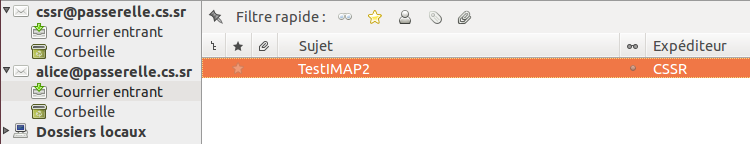
\includegraphics[scale=.7]{Thunderbird.PNG}
	\caption{\label{mua} MUA}
\end{figure}

\subsubsection{Passage à IMAPS et SMTPS}

Pour utiliser des services sécurisés, on a besoin d'implémenter SSL/TLS.
On va donc mettre en place un certificat SSL.

Il a été mentionné qu'un certificat et une clé privée avaient été générés
par Dovecot. Nous allons donc les utiliser dans la suite de la configuration.
Bien entendu, on pourrait créer "à la main" le certificat \textit{mails.crt} avec les commandes
suivantes :
\begin{verbatim}
  (passerelle)# openssl genrsa -out mails.key 2048 # Clé privée
  (passerelle)# openssl req -new -days 3650 -key mails.key -out mails.csr # Demande de certificat
  (passerelle)# openssl x509 -in mails.csr -out mails.crt -req -signkey mails.key -days 3650 
\end{verbatim}
Et on pourra supprimer le fichier \textit{mails.csr} qui n'est plus utile.
On peut également utiliser le script \textit{mkcert.sh} fourni par Dovecot.

On commence par configurer Dovecot. Dans le fichier \textit{/etc/dovecot/conf.d/10-ssl.conf} :
\begin{verbatim}
  ssl = yes # Ligne 6
  ssl_cert = </etc/ssl/certs/dovecot.pem # Ligne 12
  ssl_key = </etc/ssl/private/dovecot.pem # Ligne 13
\end{verbatim}

On relance le démon Dovecot.

Puis, on configure Postfix qui va utiliser le même certificat pour SMTPS.
Dans le fichier \textit{/etc/postfix/main.cf}, il faut ajouter :
\begin{verbatim}
  smtpd_use_tls = yes
  smtpd_tls_cert_file = /etc/ssl/certs/dovecot.pem
  smtpd_tls_key_file = /etc/ssl/private/dovecot.key
  smtpd_tls_session_cache_database = btree:${data_directory}/smtpd_scache
\end{verbatim}

Il faut également activer le démon \textit{smtps} dans \textit{/etc/postfix/master.cf}
et décommenter les lignes suivantes :
\begin{verbatim}
smtps     inet  n       -       -       -       -       smtpd
  -o syslog_name=postfix/smtps
  -o smtpd_tls_wrappermode=yes
\end{verbatim}

On relance Postfix.

\subsubsection{Tests IMAPS et SMTPS depuis Thunderbird (MUA)}

Cette fois-ci, on configure Thunderbird pour qu'il utilise
une connexion sécurisée pour le serveur entrant (IMAPS, port 993)
et pour le serveur sortant (SMTPS, port 465).
Dans les deux cas, on fournit un "mot de passe normal".
Avec une connexion sécurisée, on ne peut pas lire ce mot de passe même
si le mot de passe n'est pas chiffré.

\subsection{"Tunneliser" une connexion IMAP avec SSH}

Le protocole IMAP peut être sécurisée en utilisant la technique
de \textit{SSH tunneling}. En effet, SSH (qui est associé au port 22) est 
capable de chiffrer et déchiffrer le trafic d'autres applications sur
d'autres ports. SSH fournit alors un "tunnel sécurisé" à d'autres
connexions TCP/IP. 

Le serveur IMAP doit posséder un serveur SSH, ce qui est notre cas.
Depuis \textit{client-bsd}, on va mettre en place le tunnel :
\begin{verbatim}
  (client-bsd)# ssh -L2013:localhost:143 passerelle.cs.sr
\end{verbatim}

Le client de messagerie doit maintenant envoyer les données sur le port 2013
de sa propre machine. 

\subsection{Des messages chiffrés et signés avec GnuPG}

\subsubsection{Principe}

Il est bon de chiffrer les connexions, mais si les données
circulent par d'autres serveurs de courrier, le chiffrement
de la connexion n'est plus garanti. C'est pourquoi il faut 
envisager un chiffrement des données elles-mêmes. 

GnuPG permet de chiffrer et signer des messages électroniques. 
Chaque individu génère sa propre paire de clés : une publique et une privée.

On envoie sa clé publique à ses correspondants. Ces derniers pourront à 
terme nous écrire en toute confidentialité car ils chiffreront le message 
avec notre clé publique et nous
pourrons le lire grâce à notre clé privée.
Cependant, nos correspondants ne font pas encore confiance à notre clé publique. 
Ils doivent nous contacter (par un autre moyen de 
communication) pour comparer l'empreinte de la clé publique qu'ils ont reçu et l'empreinte
de notre clé publique. Une fois qu'ils ont confiance en la clé publique envoyée,
ils la signent avec leur clé secrète. 


Concernant la signature, nous appliquons notre clé privée sur le message que l'on souhaite
signer et nos correspondants (qui connaissent notre clé publique) pourront
vérifier que le message provient bel et bien de nous.

\subsubsection{Mise en pratique}

Pour simplifier l'utilisation de GnuPG, on utilise le plugin \textit{Enigmail} pour le MUA
\textit{Thunderbird}. Et on crée une paire de clés (et un certificat de révocation)
pour l'utilisateur \textit{alice} mais aussi pour l'utilisateur \textit{cssr}.

% --keyserver pour mettre la clef sur un serveur ... de clefs :-)
% http://wxcafe.net/archives/27

\begin{figure}[!ht]
	\centering
	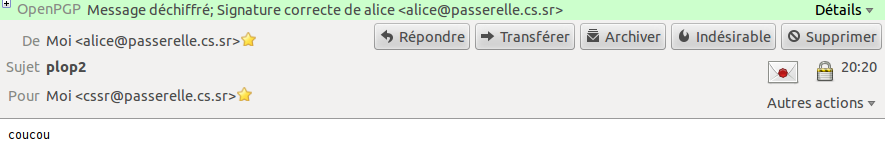
\includegraphics[scale=.5]{pgp.png}
	\caption{\label{pgp} L'utilisateur \textit{cssr} reçoit un message d'Alice qui avait été signé et chiffré}
\end{figure}

\section{Outils d'audit : OpenVAS \& Metasploit}

\section{Politique de sécurité : Flux autorisés}

En partant de la configuration suivante qui bloque le
traffic entrant, et autorise tout le traffic sortant/forwardé:
\begin{verbatim}
(passerelle)# iptables -P INPUT DROP
(passerelle)# iptables -P OUTPUT ACCEPT
(passerelle)# iptables -P FORWARD ACCEPT
\end{verbatim}

On autorise le traffic entrant venant de localhost:
\begin{verbatim}
(passerelle)# iptables -A INPUT -s 127.0.0.1 -j ACCEPT
\end{verbatim}

% http://www.frozentux.net/iptables-tutorial/chunkyhtml/x1555.html
On autorise les accès DNS sur le-serveur. Pour ce faire,
on autorise le traffic entrant venant du port $53$ sur ladite
machine, la connexion devant être \textit{ESTABLISHED}. Lors
de l'envoi de la requête DNS via UDP par un client, la connexion
sera vue comme \textit{NEW} par netfilter, puis lors de la réponse
du serveur, comme \textit{ESTABLISHED}:
\begin{figure}[!ht]
	\centering
	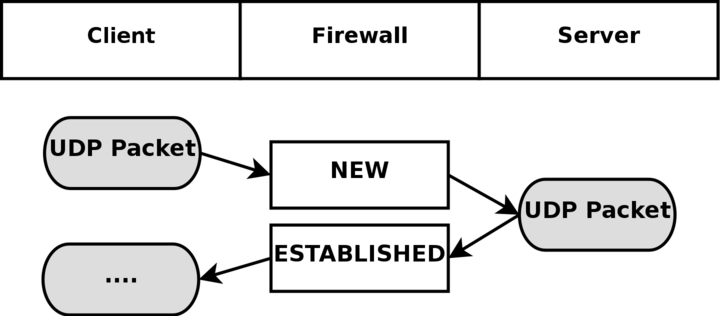
\includegraphics[scale=.5]{state-udp-connection.png}
\end{figure}

Cet état est en fait utilisé lors des échanges attendant une réponse.
Cela nous donne donc la règle suivante:
\begin{verbatim}
(passerelle)# iptables -A INPUT -i eth0 -p udp -s 192.168.1.1 --sport 53 \
     -m state --state ESTABLISHED -j ACCEPT
\end{verbatim}

On ajoute sur la chaîne INPUT le fait qu'en cas de connexion
TCP sur le port ssh, il faille accepter le traffic:
\begin{verbatim}
(passerelle)# iptables -A INPUT -p tcp --dport ssh -j ACCEPT
\end{verbatim}

D'une façon similaire, on autorise les accès HTTP et HTTPS:
\begin{verbatim}
(passerelle)# iptables -A INPUT -p tcp --dport 80 -j ACCEPT
(passerelle)# iptables -A INPUT -p tcp --dport 443 -j ACCEPT
\end{verbatim}

Enfin, pour les services emails (dans l'ordre IMAP, IMAPS,
SMTP (client/serveur) SMTPS)
\begin{verbatim}
(passerelle)# for i in 143 993 587 110 465; do \
iptables -A INPUT -p tcp --dport $i -j ACCEPT \
done
\end{verbatim}

On notera cependant que l'on ne filtre ici le traffic que sur
les ports, et pas sur le contenu. Rien n'empêche de faire passer
du traffic autre que du traffic SMTP sur le port SMTP par exemple.

% < cat appendix.tex

\newpage
\appendix

\section{Configuration d'une passerelle réseau sous FreeBSD}
Afin de voir les différences de configuration entre un Linux
et une FreeBSD, on utilise ici une topologie plus simple, mais
similaire à celle utilisée en cours.

On utilise un VMware sous un système hôte Linux ($3.7.5-1$),
faisant tourner deux machines virtuelles:
\begin{description}
	\item[FreeBSD 9.1], passerelle, disposant de deux adaptateurs
	réseaux:
	\begin{enumerate}
		\item un configuré en NAT, switch virtuel
			\textit{/dev/vmnet$8$} de l'hôte, permettant
			d'obtenir une connexion internet;
		\item l'autre en Host-Only, \textit{/dev/vmnet$1$},
			permettant d'obtenir un réseau privé;
	\end{enumerate}
	\item[Plan9 (9front-1242.62aa45fc09be)], client, doté
		d'un seul adaptateur Host-Only, configuré en t
\end{description}

En quelque sorte, la machine hôte joue ici le rôle du serveur
dans la topologie du cours, en permettant un accès aux Internets;
le réseau accessible via l'adaptateur en Host-Only permet de
créer un réseau local analogue à \textit{LAN Travaux Pratiques}.

Les parties ici présentes portant sur la configuration des services
contiennent donc des doublons par rapport à la configuration
de la passerelle sous Linux.

\subsection{Configuration de la passerelle}
\subsubsection{Interfaces réseaux}
On commence par configurer l'interface NAT, en utilisant par
exemple le serveur DHCP du switch virtuel. Ceci est normalement
déjà effectué au démarrage (cf. \textit{/etc/rc.conf}):
\begin{verbatim}
(passerelle)# dhclient em0
DHCPREQUEST on em0 to 255.255.255.255 port 67
DHCPACK from 192.168.237.254
bound to 192.168.237.132 -- renewal in 900 seconds.
(passerelle)# grep em0 /etc/rc.conf 
ifconfig_em0="DHCP"
\end{verbatim}

Puis on se connecte au réseau local, en utilisant ici une IP
statique, et l'on fait en sorte que la connection soit effective
au démmarage de la machine:
\begin{verbatim}
(passerelle)# ifconfig em1 192.168.98.2
(passerelle)# cat >> /etc/rc.conf
ifconfig_em1="inet 192.168.98.2 netmask 255.255.255.0"
^D
\end{verbatim}

On s'assure que l'on peut bien communiquer avec le système hôte
($x.x.x.1$) via les deux interfaces, et que l'on peut accéder aux
Internets:
\begin{verbatim}
(passerelle)# for i in 192.168.98.1 192.168.237.1 google.fr; do ping -c1 -q $i; done
PING 192.168.98.1 (192.168.98.1): 56 data bytes

--- 192.168.98.1 ping statistics ---
1 packets transmitted, 1 packets received, 0.0% packet loss
round-trip min/avg/max/stddev = 0.217/0.217/0.217/0.000 ms
PING 192.168.237.1 (192.168.237.1): 56 data bytes

--- 192.168.237.1 ping statistics ---
1 packets transmitted, 1 packets received, 0.0% packet loss
round-trip min/avg/max/stddev = 0.117/0.117/0.117/0.000 ms
PING google.fr (173.194.34.24): 56 data bytes

--- google.fr ping statistics ---
1 packets transmitted, 1 packets received, 0.0% packet loss
round-trip min/avg/max/stddev = 50.611/50.611/50.611/0.000 ms
\end{verbatim}

\subsubsection{IP forwarding}
On active l'IP forwarding, manuellement, puis automatiquement
au démarrage:

% http://docs.freebsd.org/doc/4.6.2-RELEASE/usr/share/doc/en_US.ISO8859-1/books/ppp-primer/x237.html
\begin{verbatim}
(passerelle)# sysctl net.inet.ip.forwarding=1
net.inet.ip.forwarding: 0 -> 1
(passerelle)# cat >> /etc/rc.conf
gateway_enable="YES"
^D
\end{verbatim}

\subsubsection{NAT}
Par défaut, le noyau de FreeBSD n'est pas configuré pour faire
du NAT; il recompiler un pépin en lui ajoutant l'option \textit{IPDIVERT}:
\begin{verbatim}
(passerelle)# cd /sys/i386/conf/
(passerelle)# cp GENERIC LOCAL
(passerelle)# cat >> LOCAL
options         IPDIVERT                # Divert packets
^D
(passerelle)# config LOCAL
Kernel build directory is ../compile/LOCAL
Don't forget to do ``make cleandepend && make depend''
(passerelle)# cd ../compile/LOCAL/ && make cleandepend && make depend && make && make install
…
kldxref /boot/kernel
\end{verbatim}

% http://www.freebsd.org/doc/en_US.ISO8859-1/books/handbook/network-natd.html
Le NAT en lui-même est géré par le démon natd, qu'il faut lancer
au démmarage, sur l'interface de sortie (em$0$):
\begin{verbatim}
(passerelle)# cat >> /etc/rc.conf
natd_enable="YES"
natd_interface="em0"
^D
\end{verbatim}

Enfin, il faut dire au bootloader de charger les modules nécessaire
pour l'IP-diverting:
\begin{verbatim}
(passerelle)# cat >> /boot/loader.conf
ipdivert_load="YES"
^D
\end{verbatim}

\subsubsection{Firewall}
On choisit arbitrairement ipfw (deux autres choix possibles: pf et ipf),
que l'on active au démmarage:
\begin{verbatim}
(passerelle)# cat >> /etc/rc.conf
firewall_enable="YES"
firewall_type="OPEN"
firewall_script="/etc/fw.sh"
\end{verbatim}

Le script fw.sh configure la table NAT et le diverting pour l'interface
\textit{em0}, tout en laissant passer tout le traffic entrant/sortant:
\begin{verbatim}
(passerelle)# cat /etc/fw.sh 
#!/bin/sh
ipfw -q -f flush
ipfw add divert natd all from any to any via em0
ipfw nat 1 config if em0
ipfw add allow ip from any to any
\end{verbatim}

Puis on indique au bootloader de charger les bons modules pour que
le pare-feu soit chargé, fonctionne avec le NAT, et soit laxiste:
\begin{verbatim}
(passerelle)# cat >> /boot/loader.conf
ipfw_load="YES"
ipfw_nat_load="YES"
net.inet.ip.fw.default_to_accept="1"
\end{verbatim}

On n'oublie pas de redémarrer pour booter sur le nouveau pépin:
\begin{verbatim}
(passerelle)# reboot
\end{verbatim}

\subsubsection{Syslogd}
Normalement, syslogd est activé par défaut. On s'assure que c'est
bien le cas, et qu'il fonctionne effectivement:
\begin{verbatim}
(passerelle)# ps aux| grep sysl
root  1140  0.0  0.6  9504 1504 ??  Ss    3:54AM  0:00.02 /usr/sbin/syslogd -s
root  1419  0.0  0.7  9636 1688  0  S+    4:20AM  0:00.00 grep sysl
(passerelle)# tail -5 /var/log/auth.log
Feb  6 03:50:41 passerelle su: cssr to root on /dev/pts/0
Feb  6 03:54:06 passerelle sshd[1237]: Server listening on :: port 22.
Feb  6 03:54:06 passerelle sshd[1237]: Server listening on 0.0.0.0 port 22.
Feb  6 03:54:29 passerelle sshd[1307]: Accepted keyboard-interactive/pam for cssr from 192.168.237.1 port 42087 ssh2
Feb  6 03:54:31 passerelle su: cssr to root on /dev/pts/0
\end{verbatim}

\subsection{Configuration du client}
On configure l'\og interface \fg\ réseau avec une IP statique,
on ajoute une route par défaut pour faire passer le traffic par
la passerelle, et on s'assure que l'on peut communiquer avec
l'extérieur:
\begin{figure}[!ht]
	\centering
	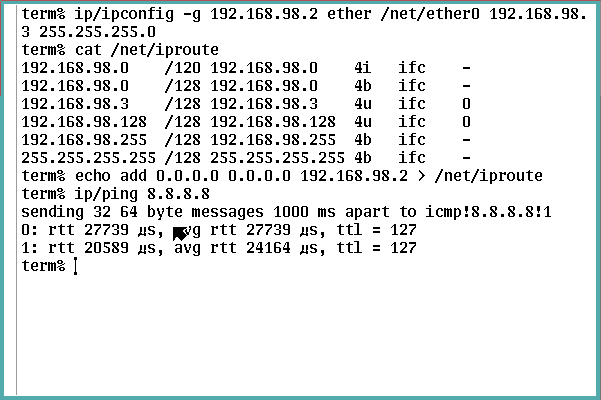
\includegraphics[scale=.5]{ipconfig.png}
\end{figure}

\section{Mise en place de services sur la passerelle}
Par manque de temps, tous les services vus en cours n'ont pas été
testés sous FreeBSD. Néamoins, pour ceux qui l'ont été,
la configuration est à quelques détails près la même dans
les deux cas. Seule la gestion du routage/firewall change vraiment,
puisque les logiciels utilisés sont dans les deux cas identiques.
Cette section est donc volontairement vide, pour éviter les doublons
avec le reste de ce document.

On notera par exemple que pour postfix, il est nécessaire de
désactiver sendmail pour éviter qu'ils ne se tappent dessus.
\end{document}
